%========================================================================
%   FileName: TechNotes.tex
%     Author: GuanHWang
%      Email: GuanHWang2011@gmail.com
% LastChange: 2014-04-18 15:41:50
%========================================================================
\documentclass[10pt,technote,onecolumn,twoside]{IEEEtran}
\usepackage[CJKchecksingle,CJKnumber]{xeCJK}
\setCJKmainfont[BoldFont={SimHei},
ItalicFont={KaiTi}]{SimSun}
\renewcommand\baselinestretch{1.2}
\usepackage{graphicx}
\usepackage[usenames,dvipsnames]{xcolor}
\usepackage{listings}
\lstset{numbers=left,numbersep=4pt,
frame=lines,framerule=1pt,basicstyle=\ttfamily\scriptsize,
}
\usepackage[bookmarksnumbered, pdfencoding=auto, 
breaklinks, colorlinks, linkcolor=red, urlcolor=ForestGreen, citecolor=magenta]{hyperref}
\usepackage{cite}
\usepackage{stfloats}
\usepackage{amssymb}
\punctstyle{plain}
\begin{document}
%\begin{CJK}{UTF8}{hei}
\title{HOG/linSVM行人检测器的OpenCV实现\\技术笔记}
\author{OnceMore2020}

%Headers
\markboth{人体检测及行为分析的研究.~TechNotes.~2014}%
{GuanHao.~电子科技大学}

%Abstract
\IEEEtitleabstractindextext{%
\begin{abstract}
HOG/linSVM行人检测器在中等分辨率和低处理速度限制的应用场景下具有明显优势。笔记参考\cite{bib1},记录了
HOG/linSVM分类器涉及到的基本理论,并记录了使用OpenCV运算库中提供的HOG描述符实现HOG/linSVM分类器的方法。
\end{abstract}

%Keywords
\begin{IEEEkeywords}
HOG特征,linSVM,分类器,OpenCV,行人检测,技术笔记.
\end{IEEEkeywords}}

\maketitle
\IEEEdisplaynontitleabstractindextext

\section{理论储备}
主要参考Dalal和Triggs在2005年的CVPR会议上提出的HOG行人检测器,即\cite{bib1}这篇“里程碑”式的论文,以及\cite{bib3},\cite{bib4}的文档。

\subsection{梯度矢量}
\textbf{梯度矢量(gradient vector)}是计算机视觉中的一个重要概念,许多视觉算法都需要引入对图像中每一个像素的梯度矢量的计算。
如下图显示的$3\times3$灰度图像,相应的像素标记字母作为标号。
\begin{figure*}[htbp]
\centering
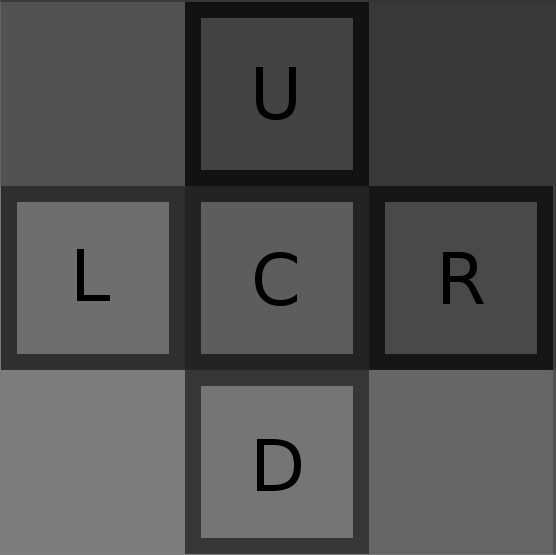
\includegraphics[width=2.6in]{gradient-3.png}
\end{figure*}

像素值在$0-255$之间,$0$表示黑色,$255$表示白色。$R-L$称为$x$方向变化率。需要注意的是,图中L像素的灰度值比R像素灰度值高,
这样计算出来会是负值,$L-R$则是正值,也称为$x$方向变化率,但是一副图像中的计算方法应当保持一致。类似的,$U-D$称为$y$方向
变化率。两个方向的变化率取值在$-255\to255$之间,不能用一个字节存储,所以需要映射到$0\to255$之间。如果将变化率用灰度值表示,则
非常大的负变化率将映射为黑色,非常大的正变化率将映射为白色。同时,我们可以得到一个梯度矢量$[R-L,U-D]$,其幅度(magnitude)和
相角(angle)计算方法如下:
\[Magnitude=\sqrt{(R-L)^2+(U-D)^2}\]
\[Angle=arctan\left(\frac{R-L}{U-D}\right)\]

梯度矢量很好地提取了边缘信息。另一方面,试想将图像的明亮度提升,即将图像中每个像素值加上同一个常数,重新计算梯度矢量会发现
和明亮度变换之前的梯度矢量一致,这种性质使得梯度矢量可以被应用到特征提取中,即本文的人体特征提取中。
\newpage
\subsection{方向梯度直方图}
如下图的一个包含行人的图像,红色框标记一个$8\times8$单元,这些$8\times8$的单元将被用来计算HOG描述符。
\begin{figure*}[!h]
\centering
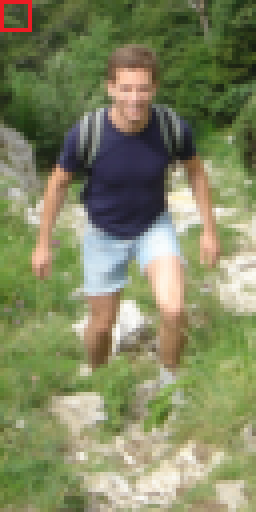
\includegraphics[width=1.6in]{hog-1.png}
\end{figure*}
在每个单元中,我们在每个像素上计算梯度矢量,将得到64个梯度矢量,梯度矢量相角在$0^\circ\to180^\circ$之间分布,我们对
相角进行分箱(bin),每箱$20^\circ$,一共9箱。具有某一相角的梯度矢量的幅度按照权重分配给直方图。例如,一个具有85度
相角的梯度矢量将其幅度的1/4分配给中心为$70^\circ$的箱,将剩余的3/4幅度分配给中心为$90^\circ$的箱。这样就得到了下面
的方向梯度直方图。
\begin{figure*}[htbp]
\centering
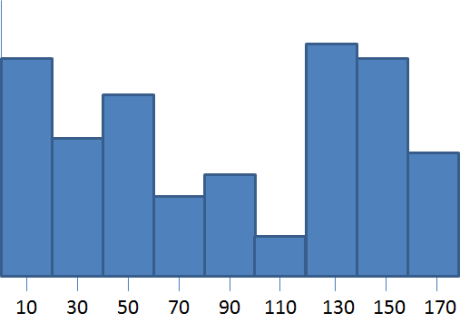
\includegraphics[width=2.5in]{hog-2.png}
\end{figure*}

上面分配幅度的方法可以减少恰好位于两箱边界的梯度矢量的影响,否则,如果一个强梯度矢量恰好在边界上,其相角的一个很小的
绕动都将对直方图造成非常大的影响。

另一方面,特征的复杂程度读分类器的影响很大。通过直方图的构造,我们将特征{64个二元矢量}量化为特征{9个值},很好地压缩了
特征的同时保留了单元的信息。设想对图像加上一些失真,方向梯度直方图的变化也不会很大,这是HOG特征的优点。同时,直方图分
箱还有其他的方法(本质上是量化)。

前面提到,对图像所有像素进行加减后梯度矢量不变,接下来引入梯度矢量的标准化,使得其在像素值进行乘法运算后仍然保持不变。
如果对单元内的像素值都乘以某一常数,梯度矢量的幅度明显会发生变化,幅度会增加常数因子,相角保持不变,这会造成整个直方图的
每个箱的幅度增加常数因子。为了解决这个问题,需要引入梯度矢量标准化,将梯度矢量除以其幅度,梯度矢量的幅度将保持1,但是其
相角不会发生变化。引入梯度矢量标准化以后,直方图各箱幅度在图像像素值整体乘以某个因子(变化对比度)时不会发生变化。

除了对每个单元的直方图进行标准化外,另外一种方法是将固定数量的单元封装成区块,然后在区块上进行标准化。Dalal和Triggs使用
$2\times2$区块(50\%重叠),即$16\times16$象素。将一个区块内的四个单元的直方图信息整合为36个值的特征($9\times4$),然后对这
个36元矢量进行标准化。标准化的算法不止上面提到的一种,\cite{bib1}中作者提供了4种标准化的方法。

区块重叠的影响是使得每个单元会在最终得到的HOG描述符中出现次数大于1次(角单元出现1次,边单元出现2次,其它单元出现4次),但
每次出现都在不同的区块进行标准化。定义一个区块位移的步长为8,则可以实现50\%的重叠。

如果检测器窗口为$64\time128$像素,则会被分为$7\times15$区块,每个区块包括$2\times2$个
单元,每个单元包括$8\times8$像素,每个区块进行9箱直方图统计(36值),最后的总特征矢量将有$7\times15\times4\times9=3780$个
特征值元素。



\section{OpenCV实现}
OpenCV提供了采用HOG特征描述符实现的人体检测的例程:\textsf{/samples/cpp/peopledetect.cpp}。
同时提供了GPU和OPENCL加速的HOG特征描述符,分别为\textsf{gpu::HOGDescriptor}和\textsf{ocl::HOGDescriptor}。
GPU加速的实现:\textsf{/samples/gpu/hog.cpp}。
OPENCL加速的实现:\textsf{/samples/ocl/hog.cpp}。

OpenCV提供的头文件在\textsf{include}文件夹中,在Ubuntu下使用源码编译OpenCV后可以在\textsf{/usr/local/include}文件夹
下找到。
\subsection{CPU HOG简单例程}
\textsf{HOGDescriptor}类定义在\textsf{object.hpp}中,一个采用\textsf{HOGDescriptor}的简单实现-
\textsf{/samples/cpp/peopledetect.cpp}代码如下:

\begin{lstlisting}[language=C++]
#include "opencv2/imgproc/imgproc.hpp"
#include "opencv2/objdetect/objdetect.hpp"
#include "opencv2/highgui/highgui.hpp"

#include <stdio.h>
#include <string.h>
#include <ctype.h>

using namespace cv;
using namespace std;

// static void help()
// {
//     printf(
//             "\nDemonstrate the use of the HoG descriptor using\n"
//             "  HOGDescriptor::hog.setSVMDetector(HOGDescriptor::getDefaultPeopleDetector());\n"
//             "Usage:\n"
//             "./peopledetect (<image_filename> | <image_list>.txt)\n\n");
// }

int main(int argc, char** argv)
{
    Mat img;
    FILE* f = 0;
    char _filename[1024];

    if( argc == 1 )
    {
        printf("Usage: peopledetect (<image_filename> | <image_list>.txt)\n");
        return 0;
    }
    img = imread(argv[1]);

    if( img.data )
    {
        strcpy(_filename, argv[1]);
    }
    else
    {
        f = fopen(argv[1], "rt");
        if(!f)
        {
            fprintf( stderr, "ERROR: the specified file could not be loaded\n");
            return -1;
        }
    }

    HOGDescriptor hog;
    hog.setSVMDetector(HOGDescriptor::getDefaultPeopleDetector());
    namedWindow("people detector", 1);

    for(;;)
    {
        char* filename = _filename;
        if(f)
        {
            if(!fgets(filename, (int)sizeof(_filename)-2, f))
                break;
            //while(*filename && isspace(*filename))
            //  ++filename;
            if(filename[0] == '#')
                continue;
            int l = (int)strlen(filename);
            while(l > 0 && isspace(filename[l-1]))
                --l;
            filename[l] = '\0';
            img = imread(filename);
        }
        printf("%s:\n", filename);
        if(!img.data)
            continue;

        fflush(stdout);
        vector<Rect> found, found_filtered;
        double t = (double)getTickCount();
        // run the detector with default parameters. to get a higher hit-rate
        // (and more false alarms, respectively), decrease the hitThreshold and
        // groupThreshold (set groupThreshold to 0 to turn off the grouping completely).
        hog.detectMultiScale(img, found, 0, Size(8,8), Size(32,32), 1.05, 2);
        t = (double)getTickCount() - t;
        printf("tdetection time = %gms\n", t*1000./cv::getTickFrequency());
        size_t i, j;
        for( i = 0; i < found.size(); i++ )
        {
            Rect r = found[i];
            for( j = 0; j < found.size(); j++ )
                if( j != i && (r & found[j]) == r)
                    break;
            if( j == found.size() )
                found_filtered.push_back(r);
        }
        for( i = 0; i < found_filtered.size(); i++ )
        {
            Rect r = found_filtered[i];
            // the HOG detector returns slightly larger rectangles than the real objects.
            // so we slightly shrink the rectangles to get a nicer output.
            r.x += cvRound(r.width*0.1);
            r.width = cvRound(r.width*0.8);
            r.y += cvRound(r.height*0.07);
            r.height = cvRound(r.height*0.8);
            rectangle(img, r.tl(), r.br(), cv::Scalar(0,255,0), 3);
        }
        imshow("people detector", img);
        int c = waitKey(0) & 255;
        if( c == 'q' || c == 'Q' || !f)
            break;
    }
    if(f)
        fclose(f);
    return 0;
}
\end{lstlisting}

程序采用了\textsf{HOGDescriptor::getDefaultPeopleDetector()}来加载默认的行人检测器,接下来的问题是怎样使用
手里已有的数据集来训练自己的分类器,这就需要了解OpenCV提供的HOG描述符的参数。

\subsection{gpu::HOGDescriptor参数}
可以在\textsf{objdetect.hpp}中找到\textsf{HOGDescriptor}的类定义:
\begin{lstlisting}{language=C++}
struct CV_EXPORTS_W HOGDescriptor
{
public:
    enum { L2Hys=0 };
    enum { DEFAULT_NLEVELS=64 };

    CV_WRAP HOGDescriptor() : winSize(64,128), blockSize(16,16), blockStride(8,8),
        cellSize(8,8), nbins(9), derivAperture(1), winSigma(-1),
        histogramNormType(HOGDescriptor::L2Hys), L2HysThreshold(0.2), gammaCorrection(true),
        nlevels(HOGDescriptor::DEFAULT_NLEVELS)
    {}

    CV_WRAP HOGDescriptor(Size _winSize, Size _blockSize, Size _blockStride,
                  Size _cellSize, int _nbins, int _derivAperture=1, double _winSigma=-1,
                  int _histogramNormType=HOGDescriptor::L2Hys,
                  double _L2HysThreshold=0.2, bool _gammaCorrection=false,
                  int _nlevels=HOGDescriptor::DEFAULT_NLEVELS)
    : winSize(_winSize), blockSize(_blockSize), blockStride(_blockStride), cellSize(_cellSize),
    nbins(_nbins), derivAperture(_derivAperture), winSigma(_winSigma),
    histogramNormType(_histogramNormType), L2HysThreshold(_L2HysThreshold),
    gammaCorrection(_gammaCorrection), nlevels(_nlevels)
    {}

    CV_WRAP HOGDescriptor(const String& filename)
    {
        load(filename);
    }

    HOGDescriptor(const HOGDescriptor& d)
    {
        d.copyTo(*this);
    }

    virtual ~HOGDescriptor() {}

    CV_WRAP size_t getDescriptorSize() const;
    CV_WRAP bool checkDetectorSize() const;
    CV_WRAP double getWinSigma() const;

    CV_WRAP virtual void setSVMDetector(InputArray _svmdetector);

    virtual bool read(FileNode& fn);
    virtual void write(FileStorage& fs, const String& objname) const;

    CV_WRAP virtual bool load(const String& filename, const String& objname=String());
    CV_WRAP virtual void save(const String& filename, const String& objname=String()) const;
    virtual void copyTo(HOGDescriptor& c) const;

    CV_WRAP virtual void compute(const Mat& img,
                         CV_OUT vector<float>& descriptors,
                         Size winStride=Size(), Size padding=Size(),
                         const vector<Point>& locations=vector<Point>()) const;
    //with found weights output
    CV_WRAP virtual void detect(const Mat& img, CV_OUT vector<Point>& foundLocations,
                        CV_OUT vector<double>& weights,
                        double hitThreshold=0, Size winStride=Size(),
                        Size padding=Size(),
                        const vector<Point>& searchLocations=vector<Point>()) const;
    //without found weights output
    virtual void detect(const Mat& img, CV_OUT vector<Point>& foundLocations,
                        double hitThreshold=0, Size winStride=Size(),
                        Size padding=Size(),
                        const vector<Point>& searchLocations=vector<Point>()) const;
    //with result weights output
    CV_WRAP virtual void detectMultiScale(const Mat& img, CV_OUT vector<Rect>& foundLocations,
                                  CV_OUT vector<double>& foundWeights, double hitThreshold=0,
                                  Size winStride=Size(), Size padding=Size(), double scale=1.05,
                                  double finalThreshold=2.0,bool useMeanshiftGrouping = false) const;
    //without found weights output
    virtual void detectMultiScale(const Mat& img, CV_OUT vector<Rect>& foundLocations,
                                  double hitThreshold=0, Size winStride=Size(),
                                  Size padding=Size(), double scale=1.05,
                                  double finalThreshold=2.0, bool useMeanshiftGrouping = false) const;

    CV_WRAP virtual void computeGradient(const Mat& img, CV_OUT Mat& grad, CV_OUT Mat& angleOfs,
                                 Size paddingTL=Size(), Size paddingBR=Size()) const;

    CV_WRAP static vector<float> getDefaultPeopleDetector();
    CV_WRAP static vector<float> getDaimlerPeopleDetector();

    CV_PROP Size winSize;
    CV_PROP Size blockSize;
    CV_PROP Size blockStride;
    CV_PROP Size cellSize;
    CV_PROP int nbins;
    CV_PROP int derivAperture;
    CV_PROP double winSigma;
    CV_PROP int histogramNormType;
    CV_PROP double L2HysThreshold;
    CV_PROP bool gammaCorrection;
    CV_PROP vector<float> svmDetector;
    CV_PROP int nlevels;


   // evaluate specified ROI and return confidence value for each location
   void detectROI(const cv::Mat& img, const vector<cv::Point> &locations,
                                   CV_OUT std::vector<cv::Point>& foundLocations, CV_OUT std::vector<double>& confidences,
                                   double hitThreshold = 0, cv::Size winStride = Size(),
                                   cv::Size padding = Size()) const;

   // evaluate specified ROI and return confidence value for each location in multiple scales
   void detectMultiScaleROI(const cv::Mat& img,
                                                       CV_OUT std::vector<cv::Rect>& foundLocations,
                                                       std::vector<DetectionROI>& locations,
                                                       double hitThreshold = 0,
                                                       int groupThreshold = 0) const;

   // read/parse Dalal's alt model file
   void readALTModel(std::string modelfile);
   void groupRectangles(vector<cv::Rect>& rectList, vector<double>& weights, int groupThreshold, double eps) const;
};
\end{lstlisting}

但是,OpenCV文档里好像找不到对应的文档,只有GPU加速和OCL加速的\textsf{HOGDescriptor}的文档,例如,
\textsf{gpu::HOGDescriptor}的类实现:
\begin{lstlisting}[language=C++]
struct CV_EXPORTS HOGDescriptor
{
    enum { DEFAULT_WIN_SIGMA = -1 };
    enum { DEFAULT_NLEVELS = 64 };
    enum { DESCR_FORMAT_ROW_BY_ROW, DESCR_FORMAT_COL_BY_COL };

    HOGDescriptor(Size win_size=Size(64, 128), Size block_size=Size(16, 16),
                  Size block_stride=Size(8, 8), Size cell_size=Size(8, 8),
                  int nbins=9, double win_sigma=DEFAULT_WIN_SIGMA,
                  double threshold_L2hys=0.2, bool gamma_correction=true,
                  int nlevels=DEFAULT_NLEVELS);

    size_t getDescriptorSize() const;
    size_t getBlockHistogramSize() const;

    void setSVMDetector(const vector<float>& detector);

    static vector<float> getDefaultPeopleDetector();
    static vector<float> getPeopleDetector48x96();
    static vector<float> getPeopleDetector64x128();

    void detect(const GpuMat& img, vector<Point>& found_locations,
                double hit_threshold=0, Size win_stride=Size(),
                Size padding=Size());

    void detectMultiScale(const GpuMat& img, vector<Rect>& found_locations,
                          double hit_threshold=0, Size win_stride=Size(),
                          Size padding=Size(), double scale0=1.05,
                          int group_threshold=2);

    void getDescriptors(const GpuMat& img, Size win_stride,
                        GpuMat& descriptors,
                        int descr_format=DESCR_FORMAT_COL_BY_COL);

    Size win_size;
    Size block_size;
    Size block_stride;
    Size cell_size;
    int nbins;
    double win_sigma;
    double threshold_L2hys;
    bool gamma_correction;
    int nlevels;

private:
    // Hidden
}
\end{lstlisting}

文档\cite{bib2}中提到(从类定义中也可以看出),GPU加速的\textsf{HOGDescriptor}类的接口和\textsf{CPU HOGDescriptor}尽量
保持一致,那么下面结合\textsf{GPU::HOGDescriptor}的API Reference来了解其参数。

\subsubsection{HOGDescriptor::HOGDescriptor}
创建HOG描述符和检测器。

函数原型:

HOGDescriptor::HOGDescriptor(Size win\_size=Size(64, 128), Size block\_size=Size(16, 16), Size block\_stride=Size(8, 8), Size cell\_size=Size(8, 8), int nbins=9, double win\_sigma=DEFAULT\_WIN\_SIGMA, double threshold\_L2hys=0.2, bool gamma\_correction=true, int nlevels=DEFAULT\_NLEVELS)

参数解释:
\begin{enumerate}
\item[$\bullet$]\textbf{win\_size}~~检测器窗口尺寸,需要和区块尺寸和区块步进对齐。
\item[$\bullet$]\textbf{block\_size}~~区块尺寸,需要和单元尺寸对齐。
\item[$\bullet$]\textbf{block\_stride}~~区块步进,需要是单元尺寸的整数倍。
\item[$\bullet$]\textbf{cell\_size}~~单元尺寸。
\item[$\bullet$]\textbf{nbins}~~分箱数量。
\item[$\bullet$]\textbf{win\_sigma}~~高斯平滑窗口参数。
\item[$\bullet$]\textbf{threshold\_L2hys}~~L2-Hys标准化参数\cite{bib5}。
\item[$\bullet$]\textbf{gamma\_correction}~~标识是否要加入伽玛校正预处理模块。
\item[$\bullet$]\textbf{nlevels}~~检测窗口增量最值
\end{enumerate}
\subsubsection{HOGDescriptor::getDescriptorSize}
返回分类需要的系数数量。
\subsubsection{HOGDescriptor::getBlockHistogramSize}
返回区块直方图的大小。
\subsubsection{HOGDescriptor::setSVMDetector}
设置线性SVM分类器的参数。
\subsubsection{HOGDescriptor::getDefaultPeopleDetector}
返回OpenCV提供的用于人体检测的分类器参数(默认检测器窗口尺寸)
\subsubsection{HOGDescriptor::getPeopleDetector48x96}
返回OpenCV提供的用于人体检测的分类器参数($48\times96$窗口尺寸)
\subsubsection{HOGDescriptor::getPeopleDetector64x128}
返回OpenCV提供的用于人体检测的分类器参数($64\times128$窗口尺寸)
\subsubsection{HOGDescriptor::detect}
进行对象检测,不进行检测窗口多尺寸缩放。

函数原型:

void gpu::HOGDescriptor::detect(const GpuMat\& img, vector<Point>\& found\_locations, double hit\_threshold=0, Size win\_stride=Size(), Size padding=Size())

参数解释:

\begin{enumerate}
\item[$\bullet$]\textbf{img}~~图像源文件,目前支持\textsf{CV\_8UC1}和\textsf{CV\_8UC4}格式的图像。
\item[$\bullet$]\textbf{found\_locations}~~检测到的目标对象边界左上角的位置。
\item[$\bullet$]\textbf{hit\_threshold}~~特征和SVM分类判定平面之间的距离门限。
\item[$\bullet$]\textbf{win\_stride}~~窗口步进,需要是区块步进的整数倍。
\end{enumerate}
\subsubsection{HOGDescriptor::detectMultiScale}
进行多尺寸窗口目标对象检测。

函数原型:

HOGDescriptor::detectMultiScale(const GpuMat\& img, vector<Rect>\& found\_locations, double hit\_threshold=0, Size win\_stride=Size(), Size padding=Size(), double scale0=1.05, int group\_threshold=2)

参数解释:
\begin{enumerate}
\item[$\bullet$]\textbf{img}~~同\textsf{HOGDescriptor::detect()}
\item[$\bullet$]\textbf{found\_locations}~~检测到的对象边界
\item[$\bullet$]\textbf{hit\_threshold}~~同\textsf{HOGDescriptor::detect()}
\item[$\bullet$]\textbf{win\_stride}~~同\textsf{HOGDescriptor::detect()}
\item[$\bullet$]\textbf{padding}~~同\textsf{HOGDescriptor::detect()}
\item[$\bullet$]\textbf{scale0}~~检测窗口增量系数
\item[$\bullet$]\textbf{group\_threshold}~~控制相似度门限,某些对象会被多个矩形覆盖,使用分组对这些矩形进行聚类。
\end{enumerate}
\subsubsection{HOGDescriptor::getDescriptors}
返回对整个图像计算得到的区块描述符。用于分类器的训练。

函数原型:

void gpu::HOGDescriptor::getDescriptors(const GpuMat\& img, Size win\_stride, \\GpuMat\& descriptors, int descr\_format=DESCR\_FORMAT\_COL\_BY\_COL)

参数解释:

\begin{enumerate}
\item[$\bullet$]\textbf{img}~~源文件
\item[$\bullet$]\textbf{win\_stride}~~窗口步进,必须是区块步进的整数倍
\item[$\bullet$]\textbf{descriptors}~~二维数组描述符
\item[$\bullet$]\textbf{descr\_format}~~描述符存储格式,有两种选择:\\ \textsf{DESCR\_FORMAT\_ROW\_BY\_ROW}(行主序)和
										\textsf{DESCR\_FORMAT\_COL\_BY\_COL}(列主序)
\end{enumerate}

\subsection{GPU加速HOG/linSVM程序实现}

% text color
%\textcolor{teal}{}

%lstling env
%\begin{lstlisting}[language=bash]
%
%\end{lstlisting}

%Single Column Floating Figure
%\begin{figure*}[!t]
%\centering
%\includegraphics[width=5in]{myfigure.pdf}
%\caption{Simulation Results.}
%\label{fig_sim}
%\end{figure*}

%double column floating figure
%\begin{figure*}[!t]
%\centering
%\subfloat[Case I]{\includegraphics[width=2.5in]{box}%
%\label{fig_first_case}}
%\hfil
%\subfloat[Case II]{\includegraphics[width=2.5in]{box}%
%\label{fig_second_case}}
%\caption{Simulation results.}
%\label{fig_sim}
%\end{figure*}

%Floating Table
%\begin{table}[!t]
%\renewcommand{\arraystretch}{1.3}
%\caption{An Example of a Table}
%\label{table_example}
%\centering
%\begin{tabular}{|c||c|}
%\hline
%One & Two\\
%\hline
%Three & Four\\
%\hline
%\end{tabular}
%\end{table}


% bibliography section
\begin{thebibliography}{99}
\bibitem{bib1}
N. Dalal and B. Triggs, “Histograms of Oriented Gradients for
Human Detection,” Proc. IEEE Int’l Conf. Computer Vision and
Pattern Recognition, pp. 886-893, 2005.
\bibitem{bib2}
Object Detection,\url{http://docs.opencv.org/modules/gpu/doc/object_detection.html}
\bibitem{bib3}
HOG PERSON DETECTOR TUTORIAL,\url{http://chrisjmccormick.wordpress.com/2013/05/09/hog-person-detector-tutorial/}
\bibitem{bib4}
GRADIENT VECTORS,\url{http://chrisjmccormick.wordpress.com/2013/05/07/gradient-vectors/}
\bibitem{bib5}
D.G.Lowe.Distinctive image features from scale-invariant keypoints.IJCV,2004.
\bibitem{bib6}
Histogram of oriented gradients,\url{http://en.wikipedia.org/wiki/Histogram_of_oriented_gradients}
\end{thebibliography}
%
%\end{IEEEbiography}
%\end{CJK}
\end{document}
